% #################################################################################
%
% LaTeX Template LaTeX for Internoise 2019
%
%
% #################################################################################
\documentclass[a4paper,12pt]{article}


%% Pick the one corresponding to your system
%\usepackage[latin1]{inputenc}
%\usepackage[ansinew]{inputenc}
\usepackage[utf8x]{inputenc}
\usepackage[T1]{fontenc}
\usepackage{times}
\usepackage[colorlinks=true,linkcolor=black,citecolor=black,urlcolor=blue]{hyperref}
\usepackage{geometry}
\geometry{top=2cm,bottom=2cm,left=2.0cm,right=2.0cm}
\pagestyle{empty}

\usepackage{titlesec}
\titleformat{\section}
{\bfseries\uppercase}{\thesection.}{1em}{}
\titleformat{\subsection}
{\bfseries}{\thesection.\thesubsection.}{1em}{}
\renewcommand{\labelitemi}{\textendash}
\renewcommand{\labelitemii}{\textendash}

\usepackage{graphicx} % used to insert the figure
\usepackage{multirow} % used for the table
\usepackage[font=it]{caption}
\usepackage{cite}
\usepackage{breakurl}
\usepackage{indentfirst}
\usepackage{amsmath, amssymb, amsfonts, bm}
\usepackage{txfonts}
\usepackage{enumitem}
\usepackage{xcolor}

\usepackage{booktabs}
\usepackage{float}

\usepackage{subcaption}
\usepackage{hyperref}

\newcommand{\simpletodo}[1]{{\color{red}#1}}

\hyphenpenalty=10000
\setlength{\emergencystretch}{3em}

\columnsep 1cm
\setlength{\parindent}{0.5cm}

\titlespacing*{\subsection}{0pt}{1.5em}{0.2em}


\renewcommand\eqref[1]{Equation~\ref{#1}}

\renewcommand{\thesection}{\arabic{section}}
\renewcommand{\thesubsection}{\arabic{subsection}}


\renewcommand{\refname}{10. \hspace{3mm} REFERENCES} 
\setlength{\footnotesep}{12pt}

\begin{document}

\begin{center}
	
\includegraphics[width=38.8mm, height=20.6mm]{logo2020.png}
\end{center}
\vskip.5cm

\begin{flushleft}
\fontsize{16}{20}\selectfont\bfseries

\color{black}Compressed Air Leakage Detection Using Acoustic Emissions with
Neural Networks
\end{flushleft}
\vskip1cm

\renewcommand\baselinestretch{1}
\begin{flushleft}

David Johnson\footnote{david.scott.johnson@idmt.fraunhofer.de}\\
Fraunhofer Institute for Digital Media Technology (IDMT)\\
Industrial Media Applications\\
Ehrenbergstraße 31, 98693 Ilmenau, Germany\\

\vskip.5cm
Jakob Kirner\footnote{jakob.kirner@idmt.fraunhofer.de}\\
Fraunhofer Institute for Digital Media Technology (IDMT)\\
Industrial Media Applications\\
Ehrenbergstraße 31, 98693 Ilmenau, Germany\\

\vskip.5cm
Sascha Grollmisch\footnote{sascha.grollmisch@idmt.fraunhofer.de}\\
Fraunhofer Institute for Digital Media Technology (IDMT)\\
Industrial Media Applications\\
Ehrenbergstraße 31, 98693 Ilmenau, Germany\\

\vskip.5cm
Judith Liebetrau \footnote{judith.liebetrau@idmt.fraunhofer.de}\\
Fraunhofer Institute for Digital Media Technology (IDMT)\\
Industrial Media Applications\\
Ehrenbergstraße 31, 98693 Ilmenau, Germany\\

\end{flushleft}

\textbf{\centerline{ABSTRACT}\\
Compressed air is utilized in many branches of industry and represents one of the most expensive energy sources of industrial plants. The efficient detection of air pressure leaks goes hand-in-hand with cost savings and increased operational reliability. Some procedures of leakage detection for pressure lines are based upon the analysis of sound emissions. Such solutions use specific ultrasonic emission patterns to detect leakage; alternatively, personnel trained to hear leaks are deployed for detection. In this paper, we evaluate the potential of airborne sound analysis in the audible hearing range for the automated detection of compressed air leakage using artificial neural networks. Therefore, a novel dataset is developed and published. It contains recordings of adjustable leakage from a pneumatic contraption with different pressure levels from several microphones at different distances. Additionally, industrial background noises were applied to simulate real-world sound environments. Using this dataset, a convolutional neural network is trained for leakage detection. The results show that leakage detection by means of airborne sound in the audible range using machine learning techniques is possible and a promising contactless automated detection method.}


\section{Introduction}

Compressed air is a common source of energy in manufacturing and other industries, and may account for up to 10\% of industrial consumption of electricity.
Compressed air systems, however, have low energy efficiency with possible energy savings from 5 to 50\%, and according to Radgen  \cite{Radgen.2001} "reducing air leaks is probably the single most important energy savings measure, applicable to almost all systems". 
Searching for leaks is typically a manual process using hand held leak "sniffers" equiped with highly directional ultrasonic microphones \cite{Radgen.2001, Schenck2019:airleakslam}, or using visual detection, which requires a leak spray \cite{Guenther2016:ultrasonic}. 
To detect leaks acoustically, an operator has to walk around the entire facility pointing a listening device towards all possible leak locations in the compressed air system. Using specialized software that visualizes and auralizes the acoustic emission, the operator must then identify if a leak is present \cite{sdt:handbook}. This process requires experienced operators, is time consuming, and may require expensive shutdowns of the production facility. The effectiveness of such an approach is dependent on the expertise and the thoroughness of the sensor operator \cite{Murvay2012:survey}. 
In addition to intensive manual labor, these methods often require shutdowns of entire facilities making leak detection an expensive process \cite{Schenck2019:airleakslam}. Identifying new techniques to improve and automate this process has the potential to lead to substantial savings in industrial energy usage and costs.

As air, or other gas, escapes a pipeline through a leak it decompresses as it enters a lower pressure environment causing turbulence. The turbulence causes an acoustic emission in the audible and ultrasonic frequencies affording the use of airborne sound based methods for leak detection\cite{Genuit.2010, Eret2012:beamform}.
Typically, the detection and localization of leaks using airborne sound is performed with ultrasonic sensors, in which case the detection process must take place in the immediate vicinity of the gas carrier or use special long distance sensors \cite{Chen.2007}. Ultrasonic microphones, however, are highly susceptible to background noise due to their low energies \cite{Eret2012:beamform}.
To overcome these challenges, this paper investigates the potential for leak detection using airborne sound in the auditory range (20 Hz - 20 kHz) with modern deep learning methods. By installing microphones around the compressed air network and automatically analyzing the airborne sound with machine learning, it might be possible to monitor a large area continuously from a distance without the need to stop production processes. Faulty lines or connections could thus be identified relatively quickly and cost-effectively. 

In recent years, the use of audible sound for predictive maintenance and automated quality control in industrial settings has grown in interest. Traditional analysis methods using audio signal processing and machine learning require expert designed hand-crafted features for fault detection. Deep learning attempts to resolve this issue by making representation learning part of the model training process \cite{Lecun2015:deep}. In industrial settings, deep learning with audio has been shown to be effective for common tasks in the research field of industrial sound analysis (ISA) \cite{Grollmisch2019:isa, Grollmisch2020:pucks, Johnson2020:robust, Grollmisch2020:embeddings}. One of the main challenges in applying deep learning methods to industrial tasks is the need for a large dataset. Obtaining well-labeled data is often expensive and time consuming, causing organizations to be reluctant to integrate deep learning into their processes. To our knowledge, there are no known datasets for the case of gas and air leak detection.

To address these gaps, the contribution of this work is to present a novel dataset for compressed air leak detection together with a convolution neural network (CNN) baseline system. CNNs have been successfully applied to tasks requiring audible sound \cite{Hershey2017:audiocnn, Grollmisch2020:pucks}. Furthermore, CNNs have shown to be more robust and less prone to overfitting than traditional feed forward networks \cite{Johnson2020:robust}. To show the potential of gas leak detection using audible sound with deep learning, we perform experiments with different types of background noise and leak conditions, as well as microphones at different distances from the leak source. The benefit of such a system, is that multiple inexpensive microphones could be placed at critical locations in the compressed air network for improved automation of the leak detection process.

% \newpage
Section \ref{sec:rw} discusses the state-of-the-art in compressed air leak detection, and industrial sound analysis using machine learning methods. Then, the design of the experimental apparatus and data acquisition process are discussed in Sections \ref{sec:app} and \ref{sec:dataset}, followed by an explanation of the baseline classification architecture in Section \ref{sec:baseline}. Sections \ref{sec:exps} and \ref{sec:res} cover the experimental design and corresponding results. Finally, Section \ref{sec:conc} concludes the paper with a discussion of the results and directions for future work.

\section{Related Work}

\subsection{Gas Leak Detection}

\subsection{Industrial Sound Analysis}

\subsection{notes}
-Ultrasonic scanning system for robotic detection \cite{Guenther2016:ultrasonic}. Uses standard statistic measures comparing sound pressure level to SNR to determine leak.
- many handheld ultrasonic systems (see above paper for some refs)
- jsn: What are the challenges of ultrasonic?

The use of acoustic sensors is a common means in the field of leakage detection.
In the field of condition monitoring for overpressure vessels surface microphones, for example, which are monitored by means of structure-borne noise emissions detect material fatigue and crack formation \simpletodo{[REF 20]}. 
In the case of airborne sound Leakage detection in practice is based on ultrasonic measuring devices, which are either installed near vulnerable areas or are portable. 
Since more complex compressed air systems usually extend over entire production plants and exact localization of high throughput turbulence leakage has the highest priority, is mobile detection solutions.
Ultrasonic sensors also enable non-destructive testing and can be performed without interrupting the ongoing operation of a system can be used. 
The turbulence leakages discussed in chapter 2.3 show a specific acoustic signature (corona) in the frequency range 38 - 42 kHz, so that appropriate measuring instruments are designed for this area.
 The converters are In addition to small-diaphragm condenser microphones \simpletodo{[REF 21]}, piezoelectric microphones are mainly used \simpletodo{[REF 22}.

Ultrasonic sensors have a strong directional characteristic, which is large main lobe and much smaller side lobes. 
In practice is referred to as the response curve. Depending on the requirements, for
individual sensors a compromise between the bundling capacity of the main lobe, the
dimensions and the side lobes [23]. 
In comparison to the directional characteristics (e.g. omnidirectional and cardioid) of microphones for audio applications however, the strong frontal directivity with accompanying sensitivity always remains
exist. 
This characteristic is essential for the ultrasonic measuring range, since sound with increasing frequencies, the damping by air absorption increases [21].

All these characteristics of the measuring devices lead to the fact that the detection process in the
in the immediate vicinity of the guest carriers. 
Due to the narrow directional characteristic all relevant areas of a gas container are scanned. 
The Occurrence of specific leakage frequencies is acoustically monitored in real time via loudspeaker
or headphone signals. 
The translation of an imperceptible ultrasonic frequency into the audible frequency range is done by a heterodyne method.
The Ultrasonic level is also translated to provide information about the leakage rate [24].


The inspection of the lines must be structured to prevent the overlooking of
to avoid leaks. If other compressed air sources such as exhaust valves or
maintenance units (see chapter 3), overlapping may occur. This competing
Ultrasound can impair the measuring accuracy or damage the sensor connected to a
Falsify the level measured in the leak [25].

2.7 Technology comparison
In the following a comparison between the leakage detection discussed in 2.6 with
ultrasound and a detection attachment with microphone for the audio range (20 Hz - 20
KHz) should be undertaken. First and foremost the applicability of the respective
technology in the foreground. The comparison is shown in Table 2.2.
The distance problem makes the ultrasonic method complex. Ultrasonic measurements
are provided at regular intervals or are used if a leakage
is to be analytically displayed and localized via system variables. Measuring microphones
in the audio range are clearly inferior in terms of measurement accuracy, but could
be placed in the service of permanent monitoring.





Due to the ability of neural networks to represent different state variables such as noise emissions, for example, can be classified with sufficient accuracy to process monitoring, there are already various experiments and studies in the field of about that. 
Already in 2004, KOTANI et al. and ZHANG et al. were able to successfully Application of NN for the detection of gas leaks by recording airborne sound in noisy environments \simpletodo{[REF 35]}. 
The results of the two studies confirmed the feasibility of process monitoring supported by ML.
Especially in ZHANG, the ability of neural networks as adaptive non-linear filters to act, highlighted \simpletodo{[REF]}. 
KOTANI has experience with recordings, which are a longer period of time. This was always done with artificially created, hole-shaped Leaks worked.
Also about the use of surface microphones for condition monitoring of larger gas containers there are current publications, in for example, where different NN models are weighed against each other \simpletodo{[REF 36]}.
However, since in this work a structure-borne sound based approach is followed, the Results not transferable to the present concept.
LIEBETRAU et al. show that a DNN with the recordings of the impact noise of turned parts can be trained to detect defective parts \simpletodo{[REF 30]}. 
In the following main part, a new experimental approach will be pursued. The main idea is to develop a dynamic leakage of adjustable leakage rates to generate and analyze.
\section{Experimental Apparatus}\label{sec:app}

We designed a compressed air network in a laboratory environment with various leak and pressure conditions to mimic real world challenges and perform experiments under controlled conditions. 
This system was used to develop the dataset for compressed air leak detection using audible sound, discussed in Section \ref{sec:dataset}.
To simulate a real factory setting, the experimental system also includes a speaker system to play background noise from real production facilities while leak sounds are being recorded.
To evaluate the effect of microphone positions, the data is recorded using microphones placed at different distances and orientations from the leak source.

\subsection{Compressed Air System}\label{subsec:app}

\begin{figure}[h]
	\centering
    \begin{subfigure}[t]{0.48\columnwidth}
        \centering
        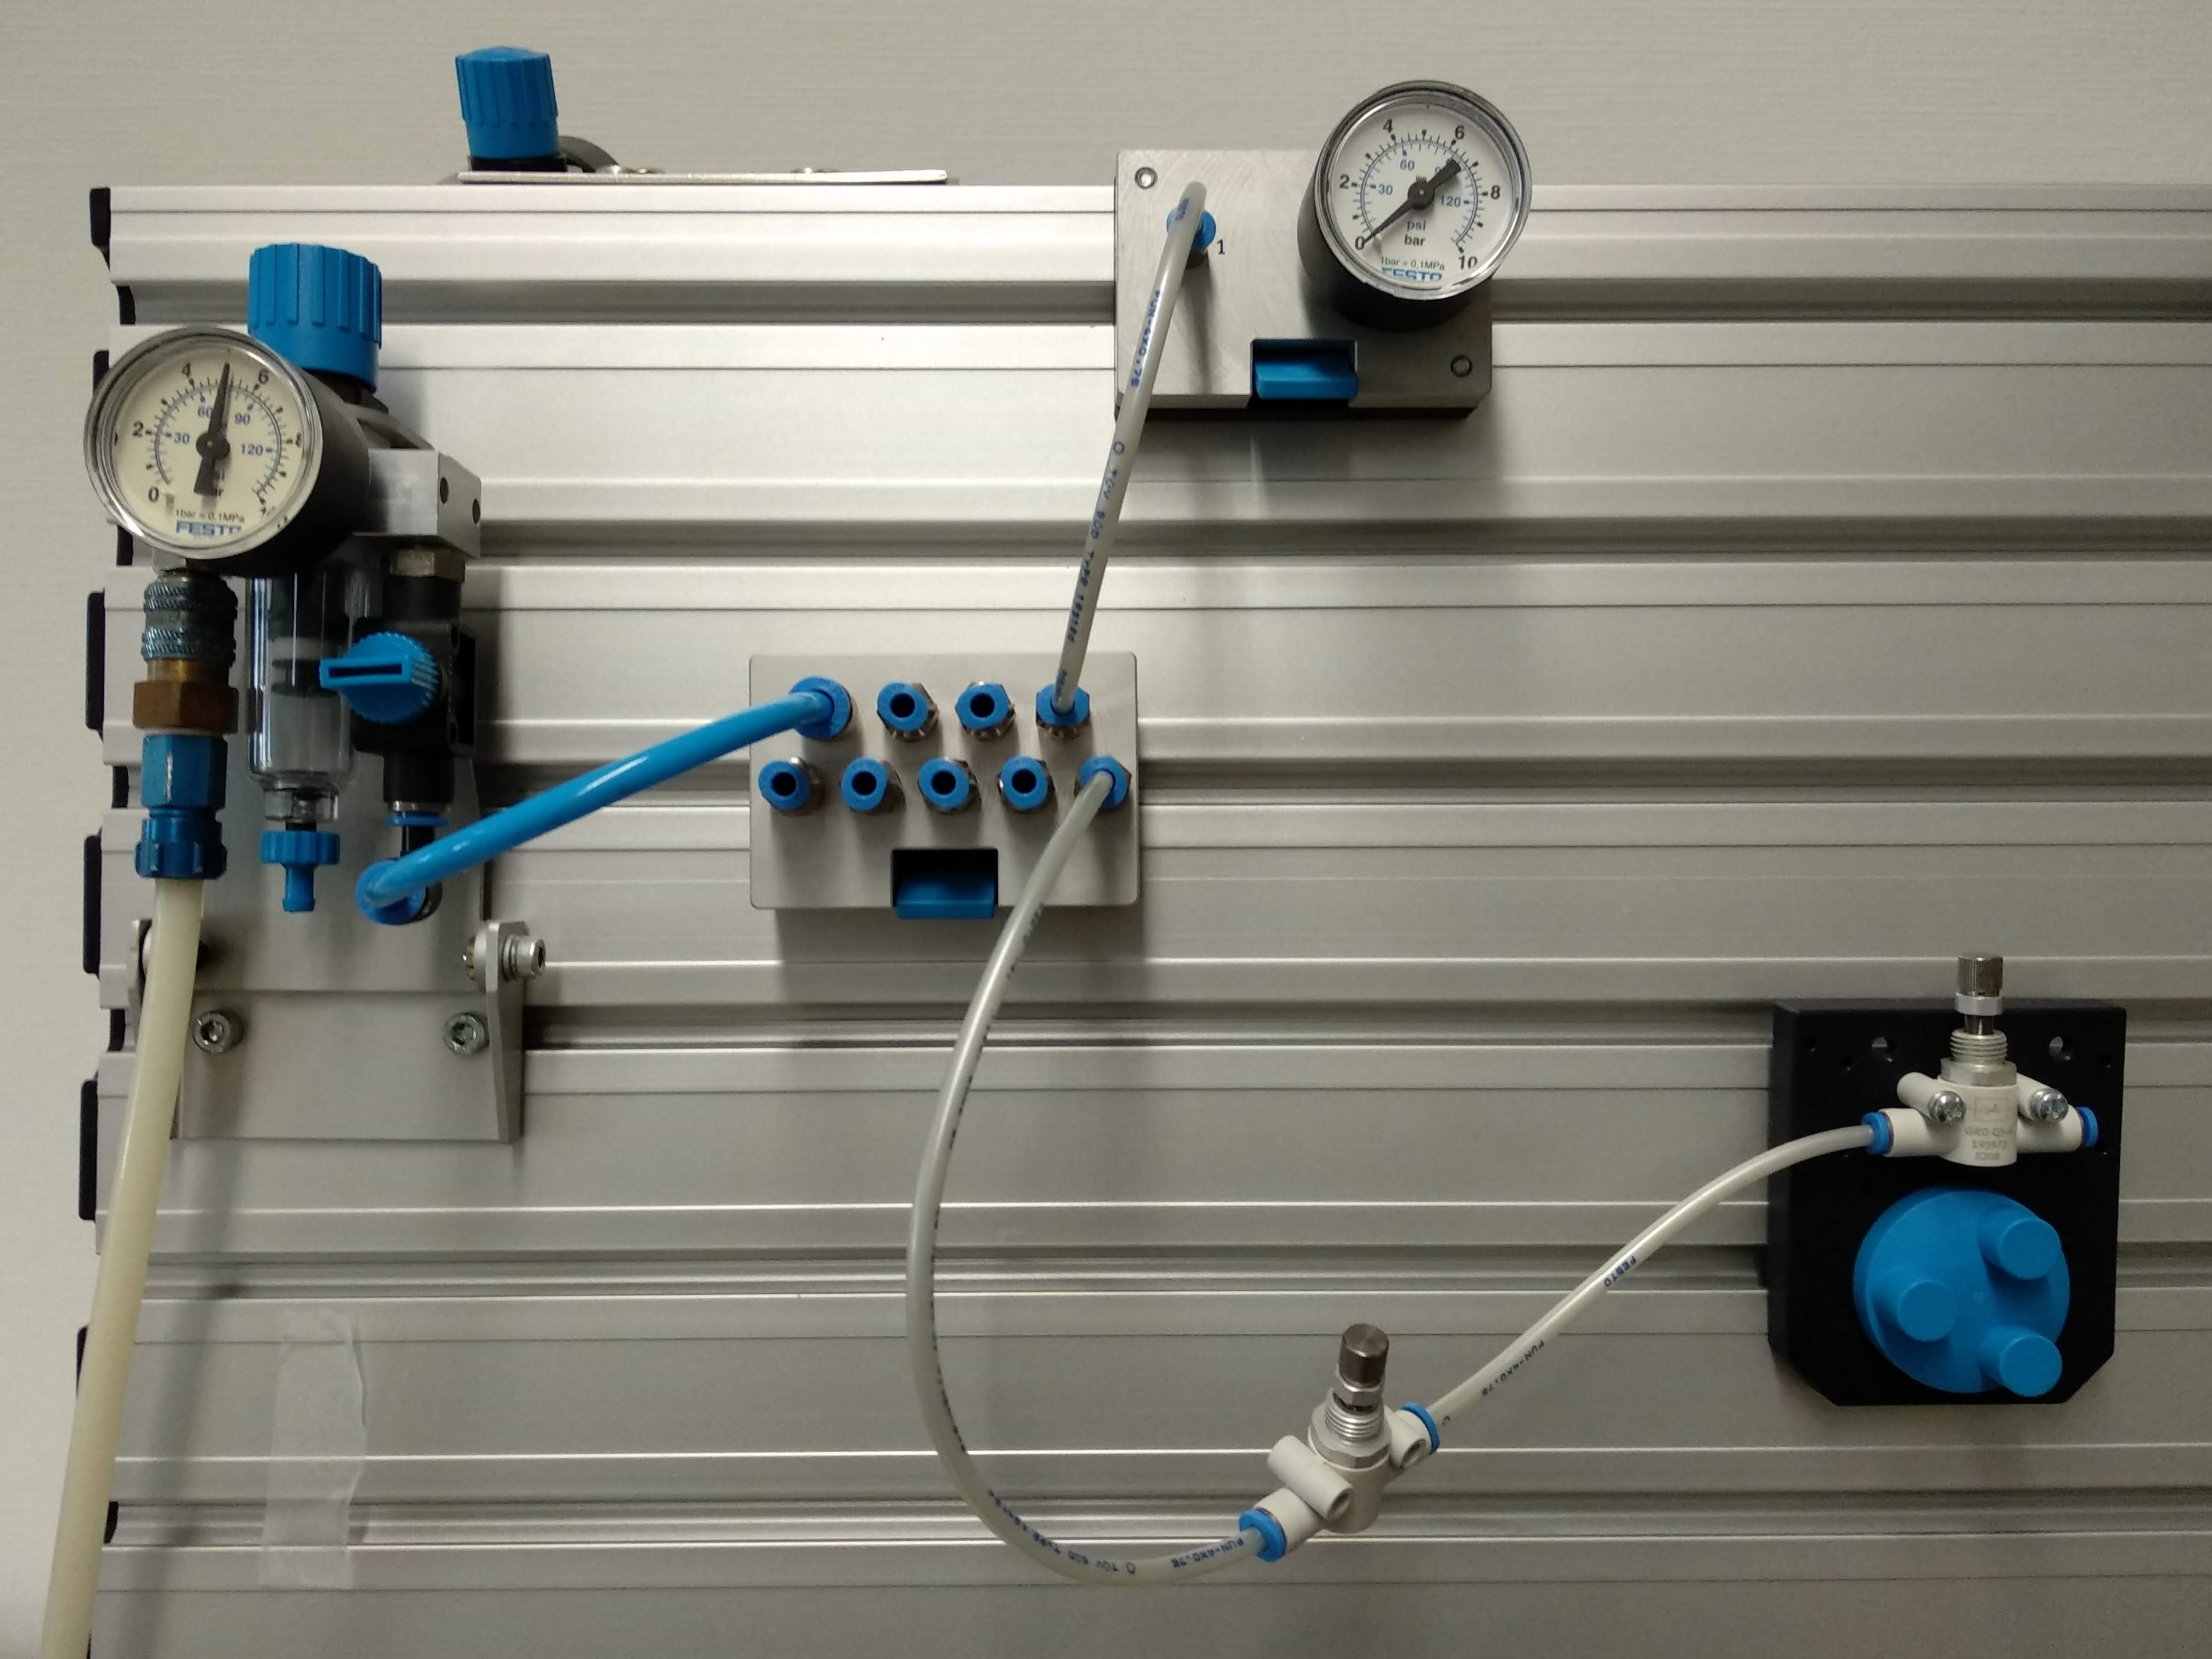
\includegraphics[width=\columnwidth]{images/apparatus_front.jpg}
        \caption{Front view}
        \label{fig:sys-front}
    \end{subfigure}%
    ~ 
    \begin{subfigure}[t]{0.48\columnwidth}
        \centering
        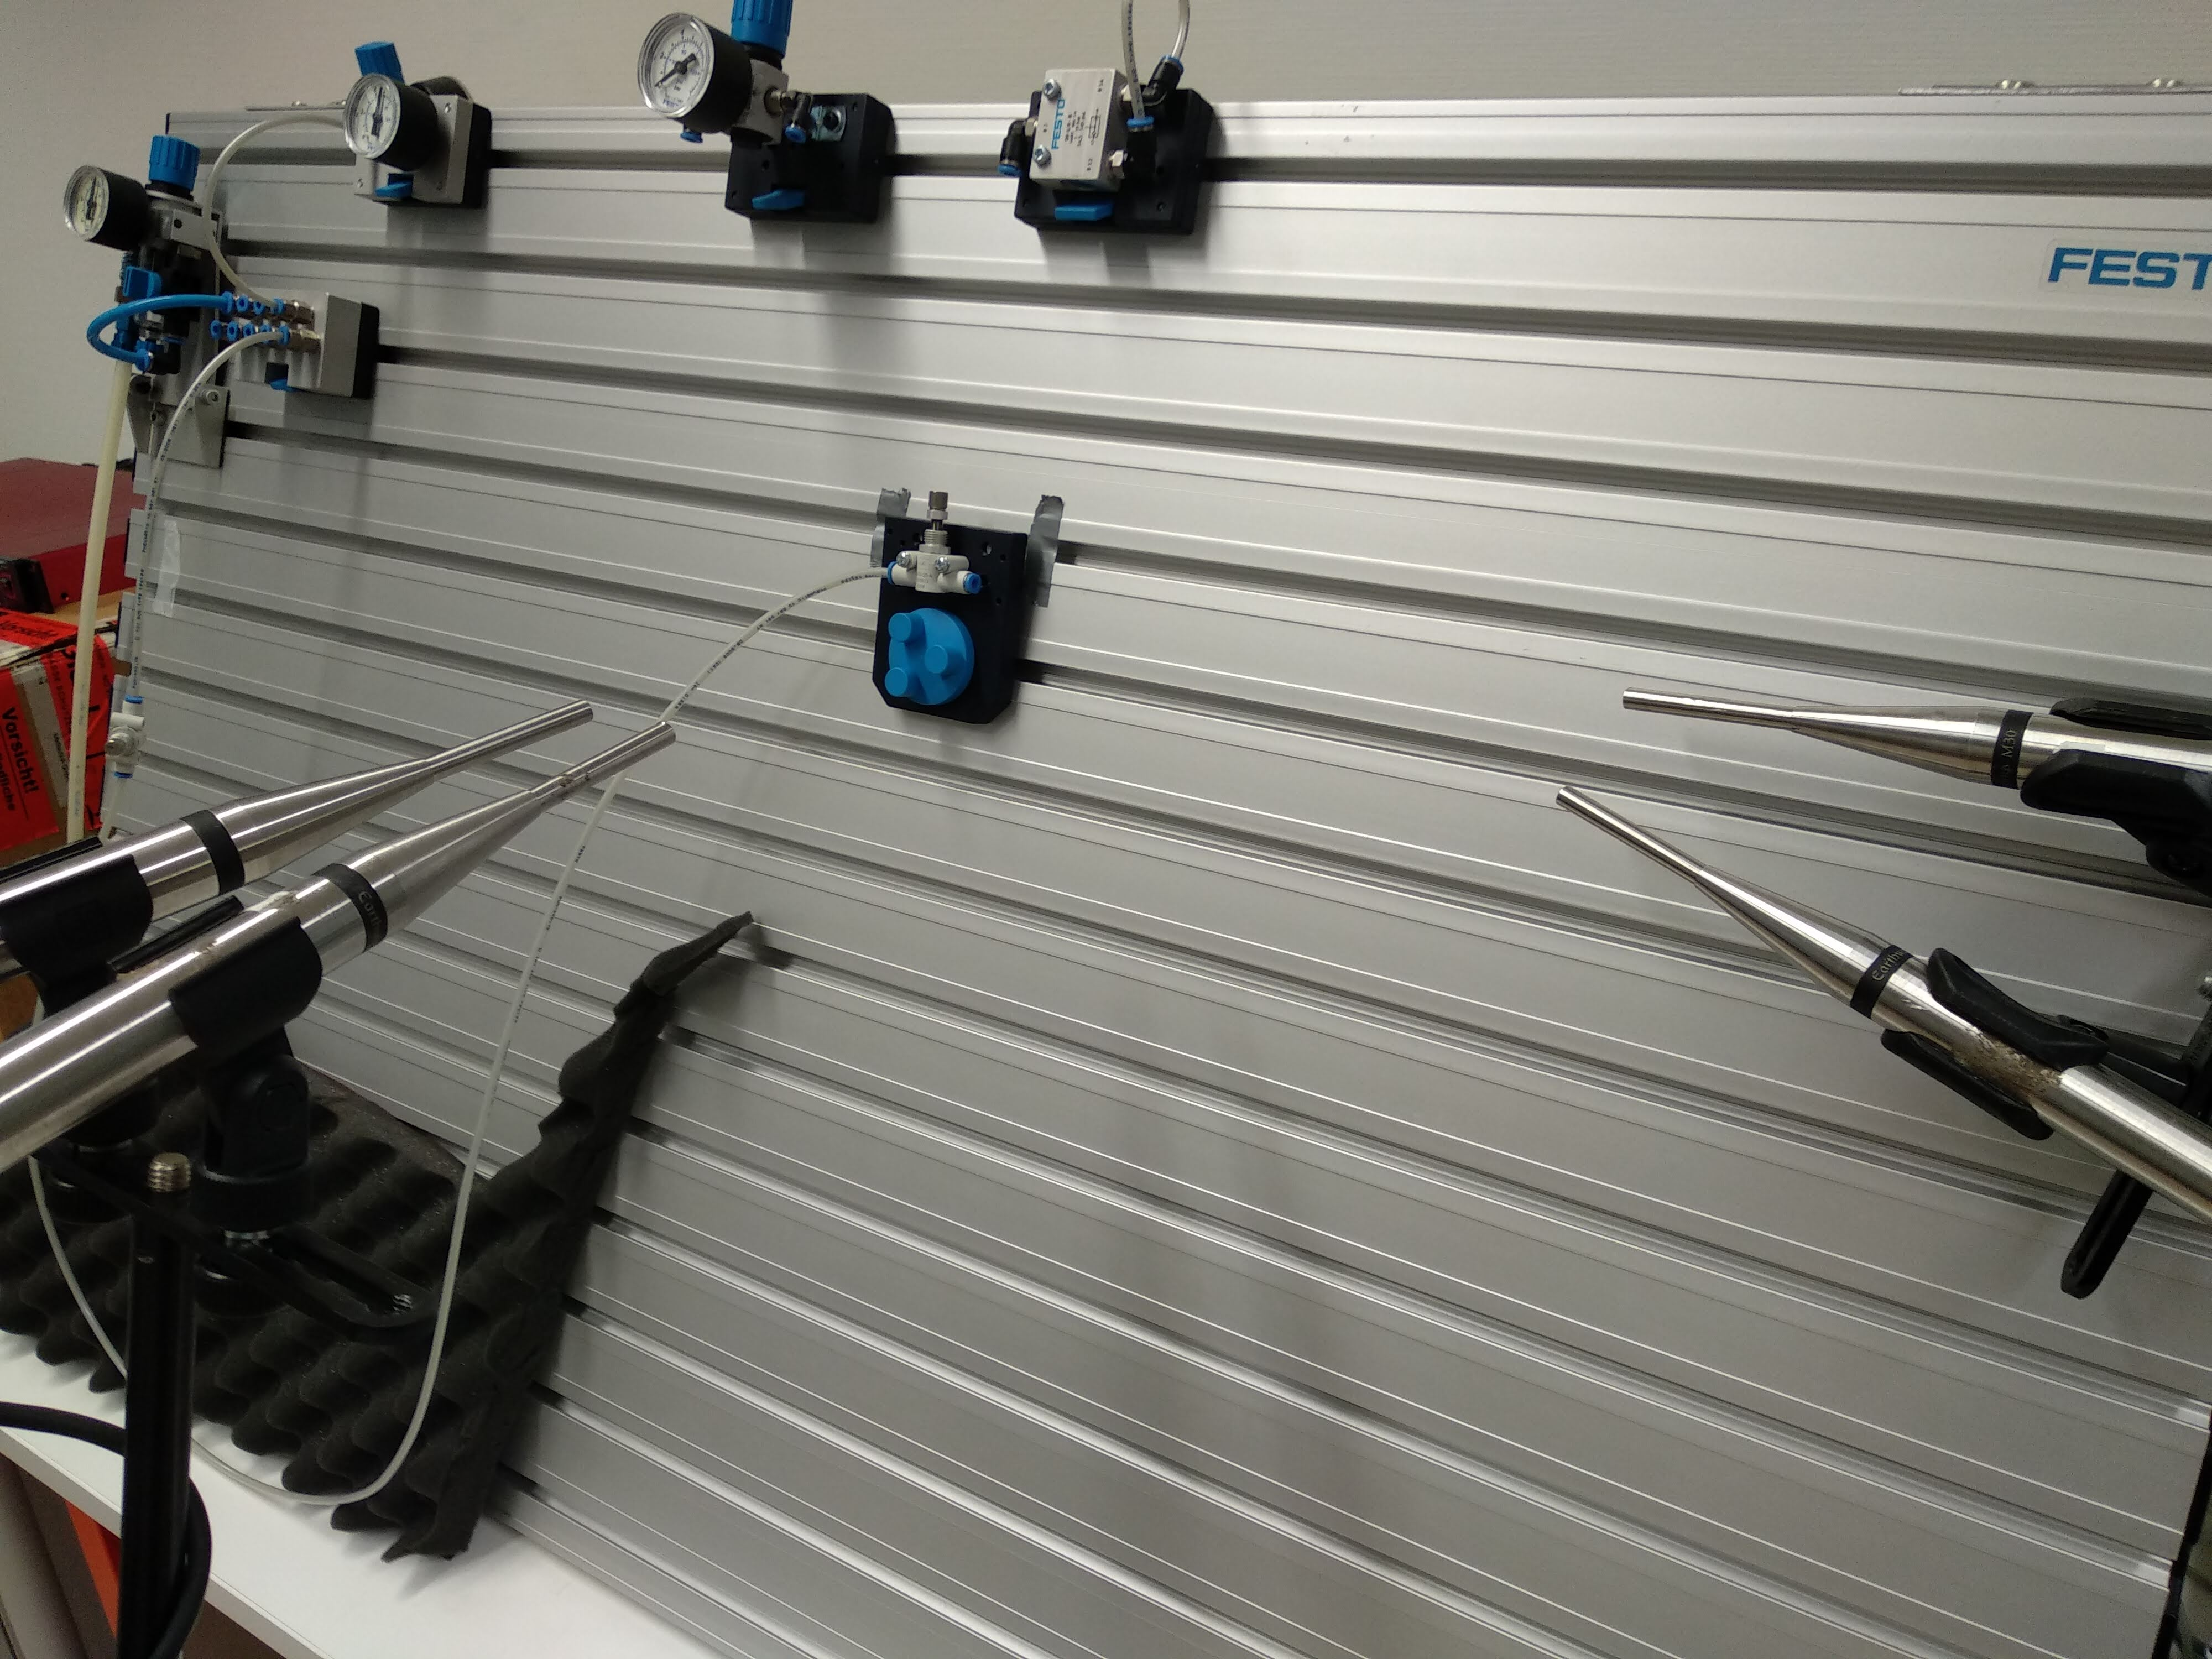
\includegraphics[width=\columnwidth]{images/apparatus_side_angle.jpg}
        \caption{Side view including microphones}
        \label{fig:sys-side}
    \end{subfigure}
	\caption{Experimental apparatus for compressed air leakage data acquisition.}
	\label{fig:sys}
\end{figure}

The experimental apparatus used for data acquisition was developed using a Festo Didactic system\footnote{\url{https://www.festo-didactic.com/int-en/}}, consisting of a tool table with a rail field that is able to be equipped with various pneumatic elements, see Figure \ref{fig:sys}. Using this modular system, a pneumatic circuit was implemented to simulate a compressed air system within a production facility. A compressed air source controls the overall pressure in the system. The leakage noises are generated by a combination of choke vents in the system. The choke vents regulate the airflow for a simulated vent leak by turning a knurled screw that generates variable flow resistance. Additionally, a damaged tube is added to the system to simulate an additional type of leak caused by a hole in the tubing.

\subsection{Microphone Configuration}

\begin{figure}[h]
    \subfloat[]{%
        \begin{minipage}[c][1\width]{0.48\textwidth}%
            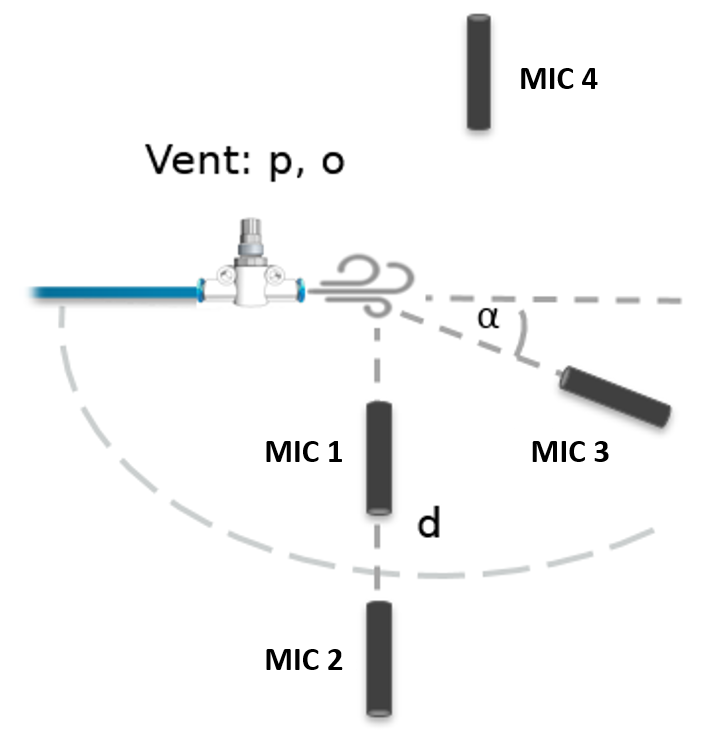
\includegraphics[clip,width=1\textwidth]{images/mic_positions.png}%
        \end{minipage}
    }
    \subfloat[]{
        \centering%
        \begin{minipage}[c][1\width]{0.48\textwidth}%
            \begin{center}
            \begin{tabular}{l l l} \toprule
                Mic & Distance ($d$) & Angle ($\alpha$)\\ \midrule
                1 & 20 cm & 90°\\
                2 & 2 m & 90°\\
                3 & 20 cm & 30°\\
                4 & Full Room & -\\ \bottomrule
            \end{tabular}
            \par
            \end{center}%
        \end{minipage}
    }
    \caption{Microphone position}
    \label{fig:mic_pos}
\end{figure}

To record acoustic emissions in the audible range, Earthworks M30 omnidirectional measurement microphones\footnote{\url{https://earthworksaudio.com/products/microphones/measurement-series/m30/}} with a frequency response in the range 3 Hz to 30 kHz are employed to record sound generated by the experimental apparatus described in Section \ref{sec:dataset}.\ref{subsec:app}.  % HACK FOR NOW
To evaluate the influence of microphone placement on leak detection, the microphones are positioned in four different locations with varying distances and angles, see Figure \ref{fig:mic_pos}. Three of the microphones (microphones 1-3) were oriented towards the leak source with an angle, $\alpha$ and distance, $d$, both described in Figure \ref{fig:mic_pos}, while the fourth microphone was placed in the center of the room near the ceiling to capture an ambient recording of the entire environment without direction.

\section{Compressed Air Leakage Dataset}\label{sec:dataset}

Using the experimental system described in Section \ref{sec:dataset}, we simulate and record a variety of conditions common to compressed air networks, including multiple leak types, pressure levels and background noises. This data set has been made publically available to fosture further research\footnote{\url{https://www.idmt.fraunhofer.de/en/publications/datasets.html}}. 

The normal pressure of the compressed air system is set to 6 bar. At this pressure level, we simulate two leak types with different acoustic characteristics: a leak that occurs at the choke vent (labeled as \textit{vent leak} throughout the rest of the paper), and a leak that occurs when a damaged tubing is installed into the system (\textit{tube leak}). A third leak is created by reducing the system pressure to 5 bar and creating a leak at the choke vent (\textit{vent low}). This introduces a leak with a lower amount of turbulence, and thus, a quieter sound.

\begin{figure}[h]
	\centering
	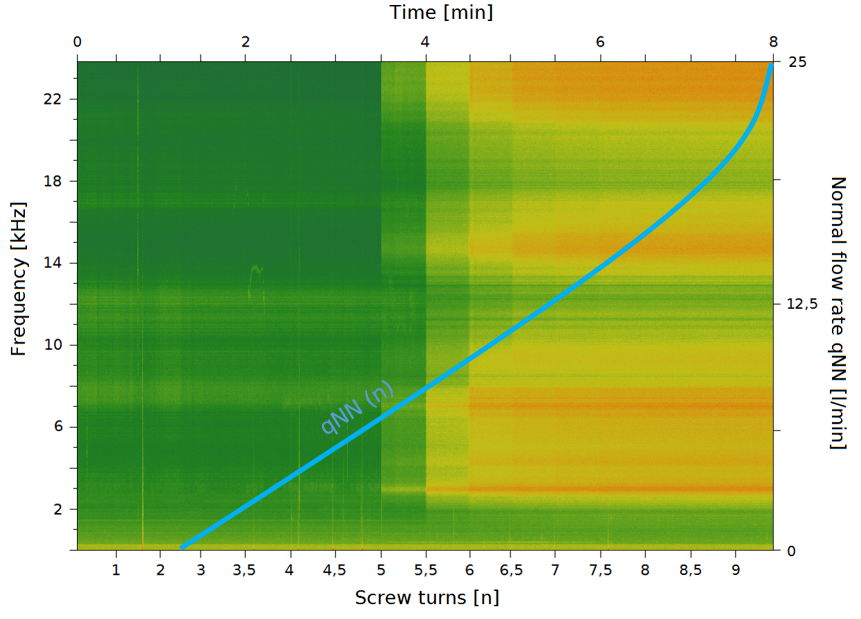
\includegraphics[width=88mm]{images/V_1_normi_qnn.png}
	\caption{Spectrogram of leakage noise from microphone position 1 with characteristic vent flow rate.}
	\label{fig:spec+qnn}
\end{figure}

To simulate normal and leak states, the amount of air escaping from the a choke vent is controlled using a knob which opens and closes the vent. Each successive turn of the knob opens the vent further, causing air to leak out. For the first three knob states, the knob is turned a complete rotation, after that the knob is turned in half rotations for each state. This is done for zero to nine turns resulting in 16 knob states. From 0 to 3 turns no air leaks from the system, and we consider these to be a non-leak states. From 3.5 to 5 turns, there is a minor leak, but the noise is not captured with our microphones, see Figure \ref{fig:spec+qnn}. In the signals recorded at 5.5 to 9 turns there is an audible acoustic emission, and this data is labeled as a leak state. 

Additionally, to mimic real-world conditions of production facilities, during recording sessions the compressed air system is recorded with one of three types of background noise. The first one is the laboratory environment noise which is introduced by the recording room itself, and contains minimal noise artefacts (called \textit{lab} throughout the rest of the paper). The other two types of noise are real-world factory noise recordings, including a typical workshop noise (\textit{workshop}, or \textit{work}) that contains aperiodic, diffuse noises, and a periodic, bolting and creaking sound created by a large hydraulic piston (\textit{hydraulic}, or \textit{hydr}). These noises are introduced into the data by playing the noise recordings on speakers in the laboratory during recording sessions. For each noise type, sessions are recorded with the noise playback at a high volume as well as low volume (indicated in the results by appending noise type with \textit{low}), which is set at 50\% of the high volume. This combination of environmental parameters results in fifteen system configurations, which can be seen in Table \ref{tab:noise-train}. Spectrograms showing the frequency content of the signals from the different leaks with the varying background noises, are shown in Figure \ref{fig:specs}. 

\begin{figure}[h]
	\centering
	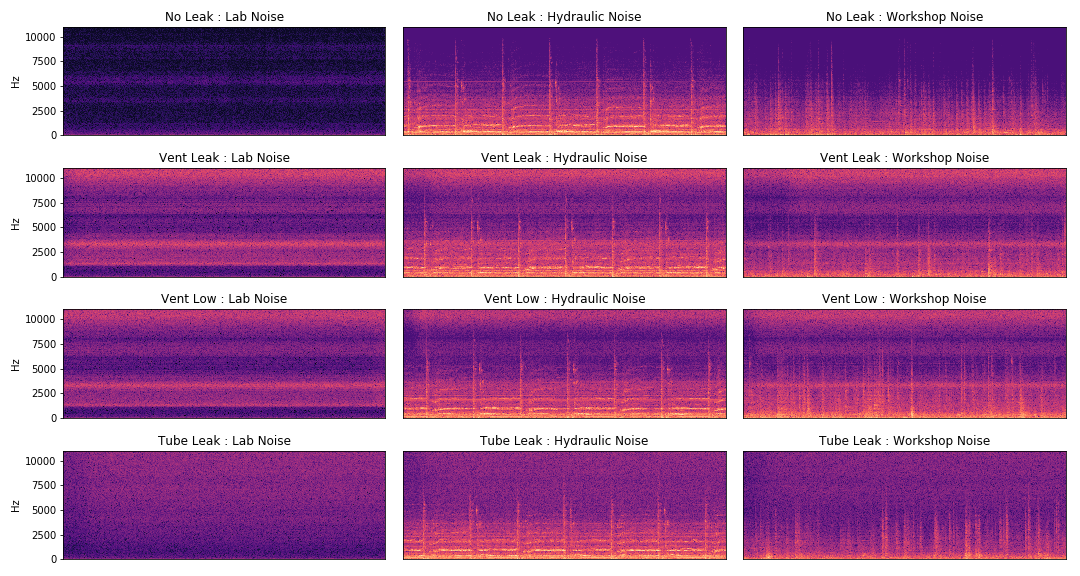
\includegraphics[width=0.95\columnwidth]{images/specs.png}
	\caption{Spectrograms from example recordings for each leak and background noise type. All data is from microphone 1.}
	\label{fig:specs}
\end{figure}

To limit bias in our data and to obtain valid results, we perform three recording sessions in which each of the 15 configurations were recorded. For each session, all four microphones are recording to ensure the data from each microphone is comparable. During the sessions, we record for 30 seconds at each each knob setting, resulting in 240 seconds of no leak recordings and 240 seconds of recordings with the specified leak for each microphone\footnote{The data from one of the sessions for the condition \textit{vent leak, workshop low} was corrupted and is not included in the full data. We mark this condition with an * in the results.}.

% \newpage
\section{Experiments}

\section{Results}

\begin{table}[h]
    \centering
    \begin{tabular}{l l l l }
    \toprule
    Condition & DNN & CNN & AUG \\ \midrule
    Base & 91.45 & 94.45 &  90.56\\
    Opening & 94.58 & 99.11 &  95.10\\
    Low Pressure &  92.92 & 96.63 & 93.54\\
    \bottomrule
    \end{tabular}
    \caption{Leave one group out cross validation}
	\label{tab:baseexps}
\end{table}

\begin{table}[h]
    \centering
    \begin{tabular}{l l l l}
    \toprule
    Condition & Noise Type & DNN & CNN \\ \midrule
    Base & Workshop &  67.70 & 68.42 \\
    Opening & Workshop & 47.52 & 59.81 \\
    Low Pressure & Workshop & 65.83 & 75.21 \\ \midrule
    Base & Hydraulic  & 39.74& 33.49  \\
    Opening & Hydraulic & 45.16 & 42.84  \\
    Low Pressure & Hydraulic & 66.72 & 58.56 \\
    \bottomrule
    \end{tabular}
    \caption{Train with normal test with low noise}
	\label{tab:baseexps}
\end{table}




%%% OLD RESULTS %%%%
% \section{Results}


% [...]
% Visible in figure \ref{fig:meanfracc} 
% - mean accuracy values of all experiments per microphone position
% - arithmetic mean (black) and max deviation (grey)
% - similar mean accuracy at similar distance 
% - odd numbers (high gain) in microphone pairs have lower mean accuracy than even numbers (low gain)

% \begin{figure}[h]
% 	\centering
% 	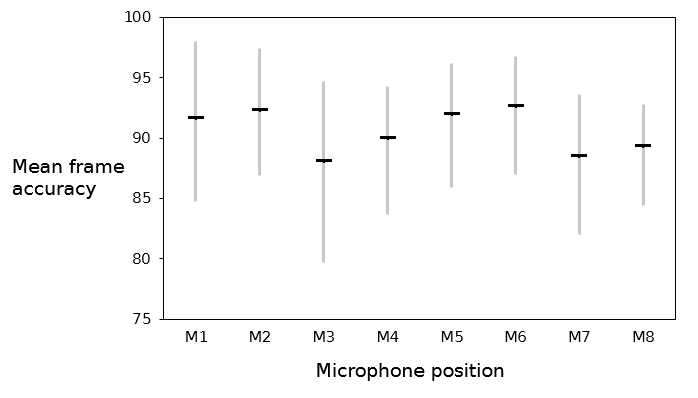
\includegraphics[width=88mm]{images/mean_frame_acc.png}
% 	\caption{Spectrogram of leakage noise from microfone position 1 with characteristic vent flow rate for 6 Bar}
% 	\label{fig:meanfracc}
% \end{figure}

% \iffalse


% \begin{figure}[h]
% 	\centering
% 	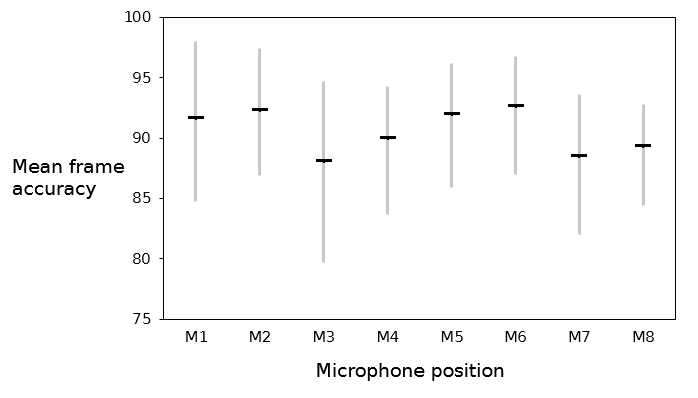
\includegraphics[width=88mm]{images/mean_frame_acc.png}
% 	\caption{Mean (frame) detection accuracy per microphone position (M)}
% 	\label{fig:mean_frame_acc}
% \end{figure}




% \begin{table}[h]
%     \centering
%     \begin{tabular}{lllllllll}
%     & 1m    & 1l    & 2m    & 2l    & 3m    & 3l    & 4m    & 4l    \\
%     \hline
%     v  & 97,97 & 96,06 & 94,65 & 94,23 & 95,19 & 94,62 & 93,22 & 91,86 \\
%     p  & 93,16 & 92,37 & 82,85 & 83,69 & 93,7  & 93,04 & 90,09 & 87    \\
%     o  & 97,81 & 97,4  & 93,65 & 93,52 & 94,83 & 96,72 & 93,63 & 88,56 \\
%     w  & 92,86 & 91,38 & 90,36 & 90,31 & 90,04 & 93,04 & 90,34 & 90,26 \\
%     h  & 92,29 & 93,69 & 88,52 & 93,51 & 96,15 & 94,88 & 89,2  & 92,55 \\
%     po & 93,54 & 93,51 & 91,76 & 90,96 & 93,18 & 94,46 & 90,52 & 92,8  \\
%     oh & 86,17 & 92,01 & 79,68 & 90,92 & 90,8  & 89,55 & 82,09 & 89,27 \\
%     ow & 86,81 & 87,86 & 85,29 & 85,4  & 87,77 & 90,61 & 85,65 & 84,37 \\
%     ph & 84,7  & 86,93 & 86,35 & 87,06 & 85,93 & 86,96 & 81,97 & 87,27 \\
%     \hline
%     \caption{Mean frame accuracy for microphone positions}
% 	\label{tab:mappingclasses}
%     \end{tabular}
% \end{table}
\section{Conclusions}\label{sec:conc}

In this article, to foster further research in data driven approaches for compressed air leak detection we present a novel dataset composed of audio recordings in the audible frequency range of a compressed air network. The dataset contains audio recordings from four microphone locations over three recording sessions. For each recording session, recordings were captured with three leak states, each with five background noise conditions, for a total of 15 recording conditions and approximately six hours of audio per microphone. Furthermore, a baseline classification system using a CNN is proposed. To evaluate the viability of a data driven approach for leak detection using audible sound , five experiments using the proposed CNN are performed. 

The results show the potential of such a system even under noisy conditions. While background noise has an effect on model performance, promising results can be achieved when the classifier is trained using data containing background noise, even with different noise types in the evaluation data. Data augmentation slightly improves the performance of models trained on clean data, but further research could clearly boost the results. A possible solution could be to augment clean data with simulated industrial noise.

The effect of microphone placement on classification performance is also evaluated with our experiments. As expected the closest microphone performs the best. Interestingly, a non-directed microphone in the middle of the room shows good performance for detection, indicating that such a microphone may be able to capture leaks in unknown locations. This indicates an ability to strategically place a microphone in a general location around a compressed air network to identify locations with possible leaks for a manual inspection, without the need to survey the entire network. Different room sizes could be considered in further research. 

% One of the aims of compressed air leak detection is to help reduce need for manual efforts by experts. Using our proposed approached, a compressed air system could be augmented with microphones directed at critical junctions in the network to automatically identify when there is a leak without the need for an expert to survey the entire compressed air network. To make this feasible, more research is needed to determine if cheap microphones could be used instead of specialized measurement microphones. Additionally, this work shows the potential to implement a monitoring approach in which a microphone is placed in a more general location to detect leaks in a larger area with one microphone. Using this method, a maintenance engineer would be alerted to the general location of the leak and then make use of a manual device to find the exact location. This would eliminate (or reduce) the need for engineers to survey the entire compressed air network looking for leaks.

With this first work on a data driven approach to compressed air leak detection, we show that a CNN can detect air leaks in noisy condition with a high rate of accuracy. While there is room for improvement, such a system could save production facilities money by reducing manually efforts to find air leaks, affording for more frequent and continuous monitoring of compressed air systems.

\section{Acknowledgements}
We gratefully acknowledge Prof. Dr.-Ing. Lena Zentner and Dirk Wetzlich from FG Nachgiebige Systeme at Technische Universität Ilmenau for providing the central infrastructure for our experiments. 

This work has been partly supported by the German Research Foundation (\mbox{BR 1333/20-1}, \mbox{CA 2096/1-1}).

\bibliography{biblio} 
\bibliographystyle{ieeetr}


\end{document}


